\documentclass{article}

% Language setting
% Replace `english' with e.g. `spanish' to change the document language
\usepackage[english]{babel}
\usepackage{float}

% Set page size and margins
% Replace `letterpaper' with `a4paper' for UK/EU standard size
\usepackage[letterpaper,top=2cm,bottom=2cm,left=3cm,right=3cm,marginparwidth=1.75cm]{geometry}

% Useful packages
\usepackage{amsmath}
\usepackage{float}
\usepackage{graphicx}
\usepackage[colorlinks=true, allcolors=blue]{hyperref}

\title{Session 7 project}
\author {
      Gkloumpos Nikolaos,
      Malthe H. Boelskift,
      Louis Ildal,
      Guillermo V. Gutierrez-Bea,
}

\begin{document}
\maketitle

\text {
      Group: 203
}

\section{Excersise 1}

SVM was used to find the boundaries between the different classes from the training set to later be used to classify the training set. The accuracy achieved with the training set is 97.92\%, and the classification results can be further examined in the confusion matrix in figure 1.
\begin{figure}[H]
      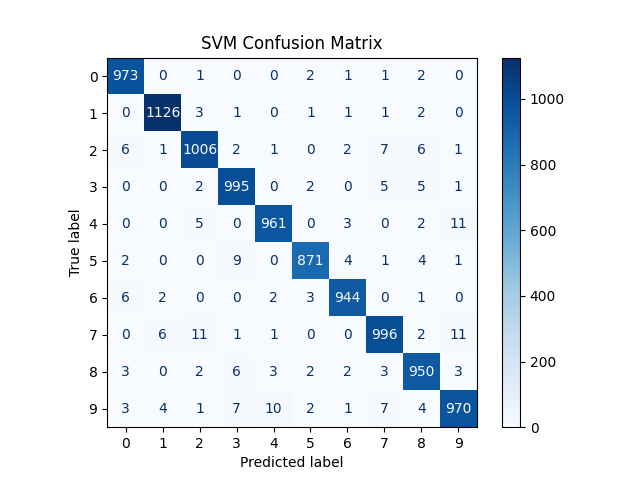
\includegraphics[width=8cm]{assets/figure1.png}
      \centering
      \caption{Confusion matrix SVM}
\end{figure}


Afterwards, SVM was applied to the dimensionally reduced datased either using PCA or LDA. The classification of the training 
set is achieved with an accuracy of 47.80\% and 57.35\% for PCA and LDA respectively. The confusion matrices of both classifications can be viewed in the following figures.
\begin{figure}[H]
      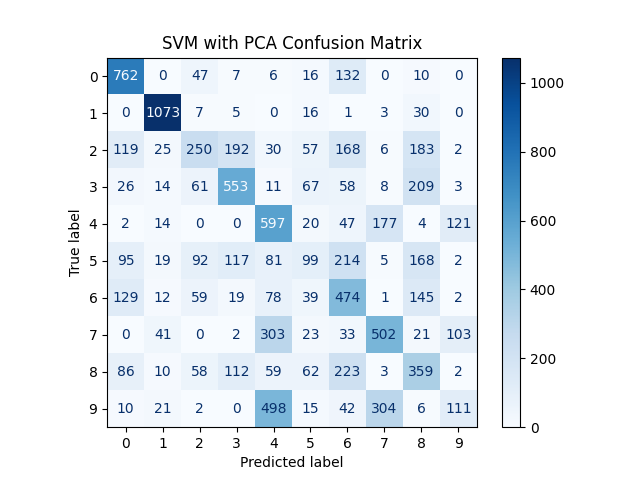
\includegraphics[width=8cm]{assets/firugre2.png}
      \centering
      \caption{Confusion matrix SVM on dimensionally reduced data using PCA} % CHeck that the figures are in correct order
\end{figure}


\begin{figure}[H]
      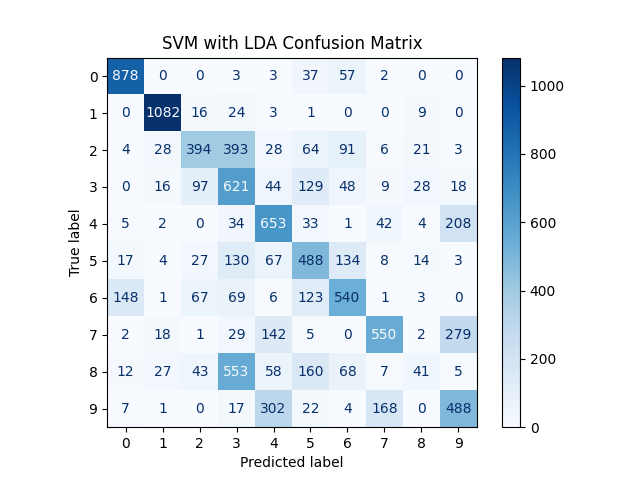
\includegraphics[width=8cm]{assets/figure3.png}
      \centering
      \caption{Confusion matrix SVM on dimensionally reduced data using LDA}
\end{figure}

\section {Environment reproduction}
To reproduce the environment used to build the excersise, follow these instructions:

\begin{verbatim}
python3 -m venv env
source env/bin/acivate
pip3 install numpy scikit-learn matplotlib
\end{verbatim}

After the above steps the program can be executed by typing

\begin{verbatim}
python3 `ProgramName.py'
\end{verbatim}

\bibliographystyle{alpha}
\bibliography{sample}

\end{document}
